\chapter{Appendix}
\section{Conclusion points assignment}\label{appendix:conclusion-point-assignment}
We outline in this section how we quantify the comparison of our approaches by assigning points to each approach for the qualitative results of the evaluation criteria. The points are real numbers of the interval $[0,\;1]$, where the highest possible point for each criterion is 1, and the lowest is 0. 

\subsection{Peformance}
%TODO: memory efficiency:
To quantize the performance discussion, we use weighted points listed in table \ref{table:performance-points} for first-time and subsequent-time performance categories. Since the maximum is $1$, the weights are chosen such that this maximum is attainable but cannot be exceeded. The best approach in a category gets the points in the first row, while the second and third-row looks at the relative difference to the best approach. What a ``small'' or ``large'' difference means is not rigorous and different for each category, i.e., a small difference for the subsequent-time build can be an order of magnitude lower than a slight difference for the first-time build. This is because the subsequent time build needs to be fast, and we penalize a difference to the best approach more. 

The approaches have the following point sums (in order of the categories in table \ref{table:performance-points}): 

\begin{itemize}
    \item NSAR: $0.35+0.1 = 0.45$
    \item BIAR: $0.25+0.35 = 0.6$
    \item Current approach: $0.1+0.65 = 0.75$
\end{itemize}
The assignment of each point is justified in the results and discussion sections (\ref{discussion:performance} and \ref{results:performance}).

\begin{table}[h!]
\centering
\begin{tabular}{||m{3.5cm}|| m{1.8cm}m{2.9cm}||} 
 \hline
 Category or \newline relative comparison & First-time build & Subsequent-time build \\
 \hline\hline
 Best approach & 0.35 & 0.65 \\ 
 Small difference to best approach & 0.25 & 0.35 \\ 
 Large difference to best approach & 0.1 & 0.1  \\ [1ex] 
 \hline
\end{tabular}
\caption{For each category, we assign points (real numbers in $[0,\;1]$) to an approach based on the relative comparison to the other approaches. There is only one ``best'' approach, and the others either have a ``small'' or ``large'' difference from this best approach.}
\label{table:performance-points}
\end{table}

\iffalse
\begin{itemize}
    \item NSAR: $0.1+0.3+0.1 = 0.5$
    \item BIAR: $0.1+0.2+0.3 = 0.6$
    \item Current approach: $0+0.1+0.6 = 0.7$
\end{itemize}
The assignment of each point is justified in the results and discussion section (\ref{discussion:performance} and \ref{results:performance}).

\begin{table}[h!]
\centering
\begin{tabular}{||m{3cm}|| m{1.8cm}m{1.8cm}m{2.2cm}||} 
 \hline
 Category or relative comparison & Memory-efficiency & First-time build & Subsequent-time build \\
 \hline\hline
 Best approach & 0.1 & 0.3 & 0.6 \\ 
 Small difference to best approach & 0.1 & 0.2 & 0.3 \\ 
 Large difference to best approach & 0 & 0.1 & 0.1  \\ [1ex] 
 \hline
\end{tabular}
\caption{For each category, we assign points (real numbers in $[0,\;1]$) to an approach based on the relative comparison to the other approaches, which means that there is only one ``best'' approach, and the others either have a ``small'' or ``large'' difference to this best approach.}
\label{table:performance-points}
\end{table}
\fi

\subsection{Security}
We quantize the security criteria with a penalty that gets subtracted from $1$ if the approach is vulnerable to a given attack target from a user group. We penalize attacks from students more than from lecturers (see table \ref{table:security-points}), for reasons discussed in \ref{discussion:security}. The weights are chosen so that each approach's worst or best assignment corresponds to the total maximum and minimum attainable points. From the discussion of \ref{discussion:security}, we conclude that the NSAR prototype is vulnerable to all attack targets and users and therefore gets $0$ points. The BIAR prototype is only vulnerable to attacks from lecturers and therefore gets $0.8$ points, whereas the current approach is safe and gets 1 point. 

\begin{table}[h!]
\centering
\begin{tabular}{||m{3cm}|| m{1.2cm} m{2.3cm}||} 
 \hline
 Attack target or user group & Host system & Other \newline environments \\
 \hline\hline
 Students & 0.4 & 0.4 \\ 
 Lecturers & 0.1 & 0.1 \\
 \hline
\end{tabular}
\caption{If an approach is vulnerable to a given attack target from a user group, then the penalty is subtracted from $1$. The result is the point assigned to the approach.}
\label{table:security-points}
\end{table}

\subsection{Developer experience}
For the developer experience, we assign weighted points to each property listed in \ref{result:UX} according to how ``important'' it is for the developer experience. The weights are chosen so that each approach's worst or best assignment corresponds to the total maximum and minimum attainable points.
Table \ref{table:devx-points} shows the points an approach receives if it fulfills the given property. In this case, it is not clear whether the approach fulfills the given property or not he receives half of the listed point. 

As mentioned in the discussion (see \ref{discussion:DevX}), the developer experience of the NSAR and BIAR prototypes is very similar for each property. Thus the point total is for both $0.9$ since they meet all properties except the third one (development and testing) since it is unclear if it is fulfilled. In contrast, the current approach has a total of $0.1$ as it does not satisfy any property except 3, where it is not fully clear whether this property is satisfied. 

\begin{table}[h!]
\centering
\begin{tabular}{||m{4cm}||ccccc||} 
\hline
 \textbf{Developer experience property number} & 1 & 2 & 3 & 4 & 5 \\
 \hline
 \textbf{Points} & 0.3 & 0.1 & 0.2 & 0.3 & 0.1 \\ 
 \hline
\end{tabular}
\caption{For each property, we assign points (real numbers in $[0,\;1]$) to an approach if it fulfills the property. The properties are listed at the beginning of \ref{result:DevX} and have the same enumeration order.}
\label{table:devx-points}
\end{table}

\subsection{User experience}
For the UX we assign weighted points to each property analogeous to the developer experience case mentioned above. Table \ref{table:ux-points} shows the points that an approach receives which is analogeous to the developer experience. The approaches have the following point sums (in order of the properties): 
\begin{itemize}
    \item NSAR: $0.15 \text{ (unclear)}+0.3+0.2+0.1 = 0.75$
    \item BIAR: $0.15 \text{ (unclear)}+0.3+0.2+0.1 = 0.75$
    \item Current approach: $0.15 \text{ (unclear)}+0+0+0.2 = 0.35$
\end{itemize}
The assignment of each point is justified in \ref{result:UX} and \ref{discussion:UX-and-DevX}. As argued in the discussion, it is unclear if each approach fulfills the first property (ease of configuration), and therefore, only half of the point is assigned in this case. 

\begin{table}[h!]
\centering
\begin{tabular}{||l||cccc||} 
\hline
 \textbf{UX property number} & 1 & 2 & 3 & 4 \\
 \hline
 \textbf{Points} & 0.3 & 0.3 & 0.2 & 0.2 \\ 
 \hline
\end{tabular}
\caption{For each property, we assign points (real numbers in $[0,\;1]$) to an approach if it fulfills the property. The properties are listed at the beginning of \ref{result:UX} and have the same enumeration order.}
\label{table:ux-points}
\end{table}

\section{Statistical test resources}\label{appendix:statistical-test}
We used the following formula to decide if the variances between two datasets $X_1$, $X_2$ with correspoding variances ${s^2_{X_1}}$ and ${s^2_{X_2}}$ are similar or not. If $max({s^2_{X_1}}, {s^2_{X_2}})/min({s^2_{X_1}},{s^2_{X_2}}) < 2$ then the variances are similar otherwise they are not. This ``rule of thumb'' is adapted from \cite{unequealVariances}, where we chose $2$ instead of $3$ as upper bound for the ratio.

\section{Additional benchmark graphs: seeded Nix store results}
\begin{figure}[h!]
  \centering
  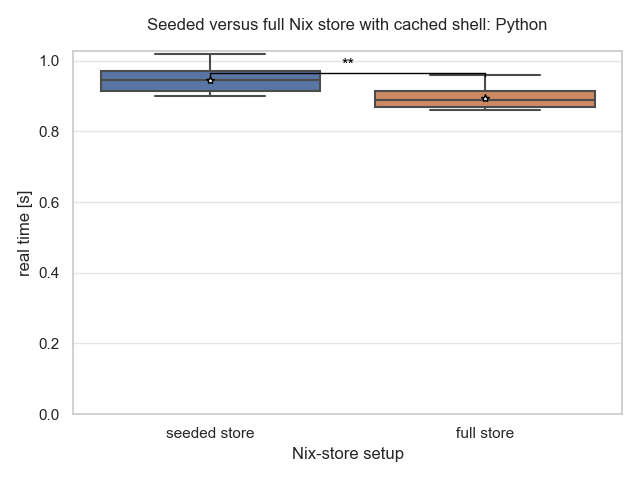
\includegraphics[width=0.75\textwidth]{thesis/graphics/nsar-plots/seeded_versus_full_nix_store_with_cached_shell:_python.png}
  \caption{The “seeded store” has a subset of the packages preinstalled to build the measured build time. The “full store” measures a subsequent build using the cached results of a first-time build with the same configuration. This graph shows the Python environment. Remarks: NSAR = nix-shell at runtime, BIAR = build image at runtime, n.s. = statistically nonsignificant difference., * = a higher number of stars(*) indicates a greater statistically significant difference.}
  \label{appendix:seeded-nix-store-python}
\end{figure}

\section{Packages included in environments for benchmarks}\label{appendix:bench-envs-packages}
The following configuration belong to the group $C_{base}$ and the specified packages are included in the benchmarks of both prototypes.
\subsection{Base packages}
\begin{lstlisting}[caption={base-pkgs.nix}, title={base-pkgs.nix}, label={base-pkgs.nix}]
{ pkgs }:
{
  inputs = with pkgs; [
    coreutils-full
    bashInteractive
    curl
  ];
}
\end{lstlisting}
\subsection{\textbf{\texttt{C++}} packages}
The Nix configuration that is used to prebuild the seeded Nix store is \nameref{cpp.nix}. 
\begin{lstlisting}[caption={cpp.nix}, title={cpp.nix}, label={cpp.nix}]
{ pkgs }:
{
  inputs = with pkgs; [
    autoconf
    automake
    bison
    flex
    binutils
    gdb
    libtool
    cmake
    strace
  ];
}
\end{lstlisting}
The Nix configuration used for benchmarking has the additional numerical library package \verb|eigen| in its configuration.

\subsection{Python packages}\label{appendix:bench-envs-packages-python}
The Nix configuration that is used to prebuild the seeded Nix store is \nameref{python.nix}. 
\begin{lstlisting}[caption={python.nix}, title={python.nix}, label={python.nix}]
{ pkgs }: with pkgs;
let
  pythonEnv = python39.withPackages (p: with p; [
    scipy
    numpy
    pandas
    termcolor
    networkx
    gnureadline
    jinja2
    matplotlib
  ]);
in
{
  inputs = [ pythonEnv ];
}
\end{lstlisting}

The Nix configuration that is used for benchmarking (see \nameref{bench-python.nix}) has \verb|scikit-learn| as an additional Python package as well as six additional OS packages compared to \nameref{python.nix}.
\begin{lstlisting}[caption={bench-python.nix}, title={bench-python.nix}, label={bench-python.nix}]
{ pkgs }: with pkgs;
let
  pythonEnv = python39.withPackages (p: with p; [
    scipy
    numpy
    pandas
    termcolor
    networkx
    gnureadline
    jinja2
    matplotlib
    
    # added Python package
    scikit-learn
  ]);
in
{
  inputs = [
    pythonEnv
    
    # added OS packages
    ncurses
    bzip2
    openssl
    sqlite
    xz
  ];
}
\end{lstlisting}

\subsection{Current approach packages}
The \verb|Python-3_8| cxEnvironment, which we used for benchmarking, has the same OS packages and Python packages as \nameref{bench-python.nix}. The \verb|GCC| configuration we used for benchmarking and comparing to our \verb|C++| environment has, apart from an additional package (\verb|eigen|), the same packages installed as \nameref{cpp.nix}. Note that the \verb|nixos/nix| base image already has the \verb|gcc| and \verb|gcc-c++| compiler installed and are therefore not in the Nix configuration. 